\chapter{Experiments and Results}\label{results}

This chapter presents the experimental results obtained in this Dissertation. The rest of the chapter is organized as follows. We first describe the corpora used for the experiments. Then we describe the experimental setup used to perform the thematic role assignment task with the Word2Vec-ESN model and the variant proposed in the previous chapter. The results obtained by the Word2Vec-ESN model, using word embeddings, are compared with $\theta RARes$ model which uses the sentences in grammatical form by replacing the semantic words with 'SW' token and localist representation of words.

\section{Corpora and pre-processing}\label{datasets}

\subsection{Corpora For TRA Task}

In order to have a fair comparison between the Word2Vec-ESN model and $\theta RARes$ model (described in section \ref{sec:xavier_model}), the performance of the models were on the  same corpus. Thus, the corpus-373, corpus-462, corpora-90582 containing 373, 462 and 90582 sentences respectively were used to perform the thematic role assignment task.  

\paragraph{Coprus-462 and Corpus-90582: } The sentence in corpus-462 and corpus-90582 was generated by Hinaut et al. using a context-free-grammer for English language and used for TRA task \cite{xavier:2013:RT}. Each sentence in these corpora have verbs which takes 1, 2, 3 clause elements. For example, the sentences, 'The man \textit{jump}', 'The boy \textit{cut} an Apple', 'John \textit{gave} the ball to Marie', have verbs with clause elements agent, agent and object, or agent, object and recipient respectively. The sentences in the corpora have a maximum of four nouns and two verbs \cite{xavier:2013:RT}. A maximum of 1 relative clause is present in the sentences; verb in the relative clauses could take 1 or 2 clause elements (i.e., without recipient). For e.g. 'The dog that bit the cat chased the boy'. Both the corpus-462 and corpus-90582 have the constructions in form:

\begin{enumerate}[noitemsep]
\item walk giraffe $<\!o\!>$ AP $<\!/o\!>$ ; the giraffe walk -s . \# ['the', 'X', 'X', '-s', '.']
\item cut beaver fish , kiss fish girl $<\!o\!>$ APO , APO $<\!/o\!>$ ; the beaver cut -s the fish that kiss -s the girl . \# ['the', 'X', 'X', '-s', 'the', 'X', 'that', 'X', '-s', 'the', 'X', '.']
\end{enumerate}

Each construction in the corpus is divided into four parts. The first part describes the meaning of sentence using semantic words (or open class words) in order of predicate, agent, object, recipient. The second part (between '$<\!o\!>$' and '$<\!/o\!>$') describes the order of thematic roles of semantic words as they appear in the raw sentence. The third part (between ';' and '\#') is the raw sentence with verb inflections (i.e. '-s') and the fourth part is the abstract representation of a sentence with semantic words removed and replace with 'X' \cite{xavier:2013:RT}.

Corpus-90582 have 90582 sentences along with the coded meaning of each sentence. This corpus is redundant; multiple sentences with different grammatical structure but the same coded meaning (see fig. \ref{fig:meaning_realtions}). In total, there were only 2043 distinct coded meanings \cite{xavier:2013:RT}. This corpus also has an additional property that along with complete coded meanings for sentences it also have incomplete meanings. For example, the sentence “The Ball was given to the Man” have no \textit{'Agent'}, and thus the meaning of the sentence is "given(-, ball, man)". The corpus also contains $5268$ pair and $184$ triplets of ambiguous sentences i.e., 10536 and 553 sentences respectively. Thus in total there were $12.24 \%$ (i.e., $ 5268 \times 2 + 184 \times 3 = 11088 $) of ambiguous sentences which have the similar grammatical structure but different coded meaning \cite{xavier:2013:RT}.

\paragraph{Corpus-373: }Apart from the corpus-462 and corpus-90582 which were artificially constructed using the context-free grammar, we also used the corpus-373. Corpus-373 includes the instructions collected from the participants interacting with a humanoid robot (iCub) in a Human-Robot Interaction study of language acquisition conducted by Hinaut et al. \cite{tra:xavier_hri}. In the study, the robot first performs one or two actions by placing the available objects to a location (e.g. left, right, middle) and the participants observes the actions. Then the participants were asked to instruct the robot again to perform the same actions in natural language. Thus the corpus contains 373 complex instructions to perform single or double actions with temporal correlation (see Action Performing task in Hinaut et al. \cite{tra:tra:xavier_hri} for more details). For example, the instruction "Point to the guitar" is a one action command whereas the instruction "Before you put the guitar on the left put the trumpet on the right" is a complex command with double actions, where the second action is specified before the first action. Thus this data is complex enough to test the learnability and generalization of the model for TRA task.

\paragraph{Pre-processing: } Recall that the corpus-462 and corpus-90582 have sentences where are verbs are represented along with inflections (suffixes "-s", "-ed", "-ing"). We preprocessed these constructions in corpus-462 and corpus-90582, to obtain the raw sentences without verb inflections.  Firstly, all the words are lowercased and then the verbs with inflections are replaced by conjugated verbs \footnote{service used to find verb conjugations: \text{http://www.scientificpsychic.com/cgi-bin/verbconj2.pl}}. The verb conjugation to be used depends on the inflection used for the verb. For example, the sentences 'The giraffe walk -s' and 'John eat -ed the apple' has been changed to 'The giraffe walks' and 'John ate the apple' respectively. This preprocessing was done because the distributed word representation captured by word2vec model already captures these syntactic relations which were imposed using verb inflection e.g $walks - walk \approx talks - talk$. We also added additional token '$<start>$' at the beginning of sentence and '$<end>$' token at the end, to mark the beginning and end of a sentence.
  
\subsection{Corpus For Training Word2Vec Model}

In this work, To train the word2vec model, we used the Wikipedia corpus\footnote{https://dumps.wikimedia.org/enwiki/latest/} ($\approx$ 14 GB) to obtain the low dimensional distributed embeddings of words. The corpus contains 2,65,8629 unique words. We chose to use Wikipedia data because we needed a general purpose dataset to get the vector representation of words. The Word2Vec model does not give good quality vector representation for words when trained over a small corpus thus a general purpose data set with billions of words is required to have good word embeddings. Thus more words we have the better the vector representation of words. Once the vector representation of words in Wikipedia data is obtained, the model can then be trained further on any our domain specific dataset (corpus-462 and corpus-90582) with more bias toward domain specific dataset (by repetition of dataset during training) to update the previously learned vector representations. 

\section{Experimental Setup}

\subsection{Obtaining Word Embeddings} \label{get_word_embeddings}

Before using the model for TRA task, we need to have the word embeddings. So in order to get the vector representation of words we first trained word2vec model on Wikipedia dataset. For training we used the word2vec model with skip-gram negative sampling (see Chapter \ref{basics} for more details) approach to obtain the word embeddings as it is claimed to produce better representation as compared to CBOW approach and is easy to train \cite{w2v:mikolov_2013_efficien, w2v:mikolov_2013_distributed}. We used the hidden layer with 50 units (desired dimensions of word embedding), and a context window of $\pm 5$. The negative sampling size is chosen to be 5 i.e. 5 noise words are chosen randomly from the vocabulary which does not appear in the context of the current input word.
As the Wikipedia corpus is huge, it contains some words like "a", "the", "in" etc. which occurs million of times. Thus the frequent words are discarded with the probabily using equation \ref{eqn:subsampling} and using a threshold of $t = 10^{-5}$. We ignored all the words which appear less than 5 times in the corpus. To update the network weights stochastic gradient is used. The initial learning rate was set to be $\alpha=0.025$, which drops to $min_alpha = 0.0001$ linearly as training progress. 

The word embeddings obtained from training on Wikipedia dataset are good enough to capture the semantic relationship between words for e.g. $vec(Paris) -vec(France) + vec(Germany) \approx vec(Berlin)$. While training the model on Wikipedia data, a vocabulary of words is created and once the vocabulary is created it is not possible to add new words to this vocabulary. However, there is a possibility that when a domain specific corpus is used to further train the word2vec model some words may not be present in previously generated vocabulary. Due to this limitation, it was not possible to get the distributed embeddings of these new words. Thus we needed to update the vocabulary of the model if the new words are not present in the vocabulary in order to facilitate the online training of Word2Vec model. Unfortunately neither C++ API \footnote{https://code.google.com/archive/p/word2vec/} nor Gensim python API \cite{w2v:gensim_api} implementation of Word2Vec supports vocabulary update once created. So, we implemented the online training\footnote{The code is adapted from-  http://rutumulkar.com/blog/2015/word2vec} of word2vec by modifying and extending Gensim API. The new words not present in existing vocabulary is added and initialized with some random weights, which can then be trained in the usual manner to have vector embeddings. Although now the vocabulary can now be updated in an online manner but the vector embedding of the newly added words has poor quality if its count in the new corpus is less. This can be improved by repetition of new dataset several times before training the model \footnote{Idea discussed on: https://groups.google.com/forum/$\#$!topic/gensim/Z9fr0B88X0w}.

So now when we have an online version of training word2vec model, we extend the word2vec model by resuming the training on the domain specific corpus (corpus-462 and corpus-90582). While updating the model on the new dataset we do not disregard any words irrespective of the count, so that we have vector embeddings of all the words in our corpus. Once trained, the vector embeddings are normalized using L-2 norm before using them. The trained word2vec model is now ready to be used with Word2Vec-ESN model.

\subsection{ESN reservoir initialization}

The size of the reservoir is one of the important parameters of ESN and is often recommended to use a bigger reservoir that can be computationally afforded provided the appropriate regularization method is used \cite{esn:practical_guide}. The bigger the size of the reservoir, the easier it is for the ESN to learn from the input signal. Thus we chose a reservoir of 1000 (until and unless specified) leaky integrator neurons with \textit{tanh} activation function. The input-to-hidden, hidden-to-hidden weights were randomly and sparsely generated using a normal distribution with mean 0 and variance 1. Thematic role assignment does not use any feedback from the readout layer, we do not use any output-to-hidden weights. The state update equations \ref{eqn:res_update} and \ref{eqn:res_state} thus changes to:

\begin{equation} \label{eqn:res_new_update}
x'(n) =\textit {tanh } ( W^{res}x(n-1) + W^{in}.u(n))
\end{equation}
\begin{equation} \label{eqn:res_new_state}
x(n) =\textit (1-\alpha) x(n-1) + \alpha x'(n)
\end{equation}

To generate the sparse weights a fixed fanout number of $F_{hh} = 10$ and $F_{ih} = 2$ was used i.e. each reservoir neuron was randomly connected to $10$ other reservoir neurons and each input neuron was connected to only $2$ other reservoir neurons. Use of fixed fanout number scales the cost of state update of reservoir linearly with increase in reservoir size \cite{esn:practical_guide}.

\subsection{Input and Ouput Coding}

As specified in chapter \ref{approach}, the Word2Vec-ESN model and its variant process the sentences differently, thus the input and output coding also differs. However, the initialization of reservoir weights remains same both the models. 

\paragraph{Word2Vec-ESN model:} A raw sentence is presented to the model, where each word in the sentence is processed across time by both word2vec model and ESN. The word2vec model outputs the $E_{v} = 50$ dimension word embedding which is then used as an input for ESN. Thus input layer of ESN has $50$ neurons. For the output coding the topologically modified but equivalent representation was used \cite{xavier:2013:RT}. Thus, the readout layer of ESN contains 24 $(4 \times 3 \times 2)$ neurons as the corpus contains sentences, having a maximum of 4 nouns each having 3 possible roles (Agent, Object, and Recipient) with respect to a maximum of 2 verbs. Each neuron in the readout layer thus codes for a role of a noun with respect to a verb. Output neuron has an activation 1 if the role is present in the sentence, -1 otherwise. When using corpus-90582 for training the number of neurons in the reservoir were raised to 5000 and also the  readout neurons are increased to 30 $(5 \times 3 \times 2)$ as there was maximum of 5 nouns in the sentences of this corpus.

\paragraph{Word2Vec-ESN model variant:} Recall that in Word2Vec-ESN model variant a raw sentence is presented to the model, where each word (argument) along with the verb (Predicate) with respect to which the word is currently processed, is input to the model across time(see section \ref{sec:model_variant}). A sentence is processed as many time as there are verbs in the sentence. The word2vec model firstly takes this argument-predicate pair as an input and outputs a vector of $E_{v} = 2 \times 50$ dimension, which is then used as an input to ESN. Thus input layer thus has $100$ neurons where first $50$ neurons encodes the vector representation of the word and remaining $50$ neurons codes for the verb with respect to which word is being processed. Unlike the model variant-1, the size of readout neurons always remains the same and contains 5 neurons each coding for a role: Predicate (P), Agent(A), Object(O), Recipient(R) and No Role(XX) for both corpus-462 and corpus-90582. When using the corpus-90582 the number of neurons in the reservoir were also increased to 3000. Readout neuron of ESN has an activation 1 if the input word-verb (argument-predicate) pair have the corresponding role, -1 otherwise. 

\subsection{Learning ESN parameters}

Echo state network have several parameters to be optimized for the proposed model to perform efficiently on thematic role assignment task. Some of the parameters like reservoir size, sparsity, distribution of non-zero weights are straightforward \cite{esn:practical_guide}. Whereas other parameters like Spectral Radius (SR), Input Scaling (IS) and Leak Rate (LR) are task dependent and are often tuned by multiple trials. Thus to identify these parameters, we performed a grid search over the parameter space. As the parameter search space can be really large, a broader grid with wider parameter ranges is first explored to find the optimal grid: grid with low sentence error for Word2Vec-ESN model and high F1-Score for the model variant. The optimal region identified previously was then used for the fine search to identify the optimal parameters \cite{esn:practical_guide}. As both the proposed model and its variant process the sentences differently and have different training objectives, the ESN parameters for both the models are optimized separately. Also, the Word2Vec-ESN model parameters are optimized separately when operated in sentence continuous learning mode and in sentence final learning mode.

To optimize the parameters, corpus-462 was used. The model was trained and tested over a range of parameters using 10-fold cross-validation method; corpus-462 with 462 sentences was randomly split into 10 equally sized subsets (i.e. each subset with $\approx$ 46 sentences). The model was trained on sentences from 9 subsets and then tested on remaining one subset. This process was repeated 10 times such that the model was trained and tested on all the subsets at least once. 


\section{Results}

\subsection{Experiment-1: Model performance on a small corpous}

In order to determine the model's capability for predicting thematic roles of the sentences using word2vec embeddings for words, we first did the experiment using limited set of sentence i.e. 26 sentences(sentence 15 to 40, in corpus-45) from corpus-45. The chosen sentences have distinct surface form (e.g. active, passive, dative-passive) and grammatical structure. This also include the sentences with single verb or double verb relative surface form \cite{}. Both the Word2Vec-model and its variant learned the sentences without any error when trained and tested on all the sentences. To test the performance and generalization capabilities of model on untrained sentences, we performed a leave-one-out cross validation, where a model is trained on 25 sentences out of 26 and tested on remaining 1 sentence.

\paragraph{Model Variant-1:} The model variant-1 with a reservoir of size 1000 units the model yielded [?] meaning error and [?] sentence error in sentence continuous learning mode and [?] meaning error and [?] sentence error in Sentence final learning mode. The results were averaged over 10 reservoir instances. For Continuous learning model the spectral radius(SR), input scaling (IS) and leak rate($\alpha$) were identified as $SR=[?], IS=[?], \alpha=[?]$.` Whereas for Sentence final learning mode the $SR=?, IS=?, \alpha=?$. The ESN parameters for which the optimized results are identified are found by exploration of parameter space. As one may note that difference in training and test error for both meaning and sentence error is large. This indicates the model is overfitting on the dataset. However, it is not surprisring because the dataset contains limited examples, which constrained model to generalize well. As this experiments remains a toy demonstration we will explore the generalization capabilty of the model in section \ref{exp-2} .

\paragraph{Model Variant-2:} The model Variant-2, on the other hand, with a reservoir of size 600 neurons, produced the classification scores [write score here] during cross-validation. 

\subsection{Experiment-2: Generalization Capabilities} \label{exp-2}

In the previous experiment we demonstrated the performance of the model with the limited set of sentences where the results suggested that the model is probably overfitting and not generalizing on the unseen sentences. So in order to test the generalization capability of the model, we examined the model's behaviour with an extended corpus of 462 sentences (see corpus-462 in \ref{datasets}) using 10-fold cross validation. 

\paragraph{Word2Vec-ESN:} We initially trained and tested the model on all the 462 sentences. The model learned the full corpus-462 with $0.54\%$ meaning error and $1.51\%$ sentence error in SCL mode and $0.14\%$ meaning error and $0.43\%$ sentence error in SFL mode. Using the 10-fold cross validation, the model generalized to $7.82\% (\pm 1.59\%) $ meaning error and $20.65\% (\pm 2.79\%)$ sentence error in SCL mode with spectral radius (SR), input scaling (IS) and leak rate(LR) of $2.4$, $2.5$ and $0.07$ respectively. Whereas in the SFL mode with reservoir parameters $SR = 2.2$, $IS = 2.3$ and $LR = 0.13$, the optimal meaning and sentence error were observed as $8.68\% (\pm 1.26\%)$ and $23.69\% (\pm 1.17\%)$ respectively.

We compared the performance of Word2Vec-ESN model with $\theta RARes$ model which takes the sentences in grammatical form and words are represented in localist fashion. As illustrated in table \ref{tab:corpus-462_errors}, during testing, we observed an improvement of $11.48 \%$ sentence error in SCL mode with Word2Vec-ESN langugae model whereas meaning error remained almost equivalent in both the Word2Vec-ESN and $\theta RARes$ models. In SFL mode, using Word2Vec-ESN model, both meaning and sentence errors dropped nearly by $1 \%$. One can also notice that with Word2Vec-ESN model, the performance gain is more in SCL mode as compared to SFL mode whereas it was vice-versa in $\theta RARes$ model. 

%NOTE: 08/09/2016 results are copied after the simulation and are final, no need to change.
\begin{table}
\centering
\begin{threeparttable}
\caption{Mean and standard deviation of meaning and sentence error on train and test set of coprus-462 in different learning modes.}
\label{tab:corpus-462_errors}
\rowcolors{2}{white}{gray!25}
\begin{tabular}{llcccccccc}
  \toprule
  \hiderowcolors   
  &  & \multicolumn{4}{c}{Word2Vec-ESN} & \multicolumn{4}{c}{$\theta RARes$} \\
  \cmidrule(lr){3-6}   \cmidrule(lr){7-10}
  
  &  & \multicolumn{2}{c}{Corpus 462} & \multicolumn{2}{c}{462 scrambled} & \multicolumn{2}{c}{Corpus-462} & \multicolumn{2}{c}{462 scrambled} \\
  \cmidrule(lr){3-4} \cmidrule(lr){5-6}  \cmidrule(lr){7-8} \cmidrule(lr){9-10}  
  
  
   						& 		& ME 	& SE 		& ME 	& SE 			& ME 	& SE		& ME 	& SE 		\\
  \midrule
  \showrowcolors
  \textbf{SCL\ train} 	& mean 	& 0.541 & 1.515  	& 7.312  & 30.303	 	& 0.123 & 1.207 	& 4.813  & 20.433	\\
   			    		& std 	& 0.000 & 0.000 	& 0.000  & 0.000 		& 0.029 & 0.297 	& 0.299  & 1.251	\\
   			    		
  \textbf{SCL\ test} 	& mean  & 7.826 & 20.652 	& 69.761 & 99.130 		& 7.433 & 32.130 	& 74.154 & 99.891	\\
  			   			& std  	& 1.598 & 2.792 	& 1.462  & 1.064  		& 0.524 & 1.353 	& 0.802  & 0.146	\\
  			   			
  \textbf{SFL\ train} 	& mean 	& 0.144 & 0.432 	& 9.148  & 31.168 		& 0.000 & 0.000 	& 0.000  & 0.000	\\
  				 		& std 	& 0.000 & 0.000 	& 0.000  & 0.000 		& 0.000 & 0.000 	& 0.000  & 0.000	\\
  				 		
  \textbf{SFL\ test}	& mean  & 8.686 & 23.695 	& 67.548 & 99.347 		& 9.178 & 24.370 	& 73.391 & 99.913	\\
  			  			& std 	& 1.265 & 1.170		& 1.971  & 0.996  		& 0.574 & 1.192 	& 0.962  & 0.106	\\
  \bottomrule
\end{tabular}
\begin{tablenotes}
\small
\item 
Meaning (ME) and Sentence error (SE) in different learning modes with Word2Vec-ESN model using distributed word embeddings and $\theta RARes$ \cite{xavier:2013:RT} model which uses grammatical form and localist representation of words of sentences. The errors are given in percentage. SFL:Sentence Continuous learning; SFL: Sentence Final Learning; std: Standard Deviations. Simulations were done with reservoir of 1000 neurons.
\end{tablenotes}
\end{threeparttable}
\end{table}
	
\paragraph{Word2Vec-ESN Variant:} The word2vec-ESN model variant with a reservoir of size 1000 neurons when trained and tested on all 462 sentences of corpus-462, the model learned to label the argument-predicate pairs in the sentences with an Accuracy (Ac), Precision (Pr), Recall (Re) and F1-Score (F1) of $97.38\%$,  $97.48\%$, $92.28\%$, $94.64\%$ respectively. When the model variant was tested using 10-fold cross validation for generalization, we observerd Ac = $97.10\% (\pm 0.04\%)$, Pr = $96.76\% (\pm 0.08\%)$, Re = $91.78\% (\pm 0.08\%)$ and F1 = $93.99\%(\pm 0.09\%)$ with $ IS=1.15, SR = 0.7, LR = 0.1$. The marginal difference between the training and cross validation scores indicates that the model variant is generalizing well on untrained sentences and is not overfitting. 

In order to see the effect of using distributed word embeddings on model variant we  also performed the simulations using grammatical form of sentences with localist word representations. When using GF and localist word representations, the model produced Pr = $80.66 \% (\pm 0.22\%)$, Re = $84.69 \% (\pm 0.13\%)$, F1 = $82.23 \% (\pm 0.15\%)$ during training and Pr = $78.37 (\pm 0.40\%)\% $, Re = $81.56 \% (\pm 0.33\%)$, F1 = $79.51 \% (\pm 0.34\%)$ during cross-validation. The precision, recall, and the f1-score of invidiual roles produced by model variant are reported in table \ref{tab:classsification-scores-21} 

%NOTE: 08/09/2016 results are copied after the simulation and are final, no need to change.
\begin{table}
\centering
\begin{threeparttable}
\caption{Training and testing classification scores for individual roles when using Word2Vec-ESN model variant.}
\label{tab:classsification-scores-21}
\rowcolors{2}{gray!25}{white}
\begin{tabularx}{\textwidth}{@{}llYYYYYYY@{}}
\hiderowcolors
\toprule
  &  & \multicolumn{3}{c}{word2vec vectors} & \multicolumn{3}{c}{GF \& localist vectors}& \\  
\cmidrule(lr){3-5}   \cmidrule(lr){6-8}
   
Role 				& 			& Pr   & Re  & F1 		& Pr  &  Re & F1 		&  Support  \\
\showrowcolors
\midrule
               
\textbf{Agent}		&test 		& 0.92 & 0.79 & 0.85 	& 0.66 & 0.62 & 0.64	& 888 \\
					&train  	& 0.94 & 0.80 & 0.86 	& 0.71 & 0.66 & 0.69	& 892 \\
\textbf{Object}		&test 		& 0.95 & 0.81 & 0.88 	& 0.62 & 0.65 & 0.64	& 791 \\
					&train  	& 0.96 & 0.82 & 0.88 	& 0.67 & 0.69 & 0.68	& 794 \\
\textbf{Recipient}	&test 		& 1.00 & 1.00 & 1.00 	& 0.69 & 0.91 & 0.78	& 383 \\
					&train  	& 1.00 & 1.00 & 1.00 	& 0.68 & 0.97 & 0.80	& 384 \\
\textbf{Predicate}	&test		& 1.00 & 1.00 & 1.00 	& 0.94 & 0.92 & 0.93	& 888 \\
					&train  	& 1.00 & 1.00 & 1.00 	& 0.98 & 0.94 & 0.96	& 892 \\
\textbf{No Role}	&test 		& 0.97 & 1.00 & 0.99 	& 0.97 & 0.96 & 0.96	& 9785 \\
					&train  	& 0.97 & 1.00 & 0.99 	& 0.98 & 0.97 & 0.97	& 9823 \\
\bottomrule
\end{tabularx}
\begin{tablenotes}
\small
\item Comparision of training and cross validation scores for each output roles predicted by the model. Support for each role: actual number of instance, is also shown in last column. Simulation were done using 1000 reservoir neurons and parameters: SR = 0.7, IS = 1.15, LR = 0.1.
\end{tablenotes}
\end{threeparttable}
\end{table}

% analyse table and confusion matrix
[Confusion matrix to be analyzed]

\begin{figure}[hbtp]
\centering
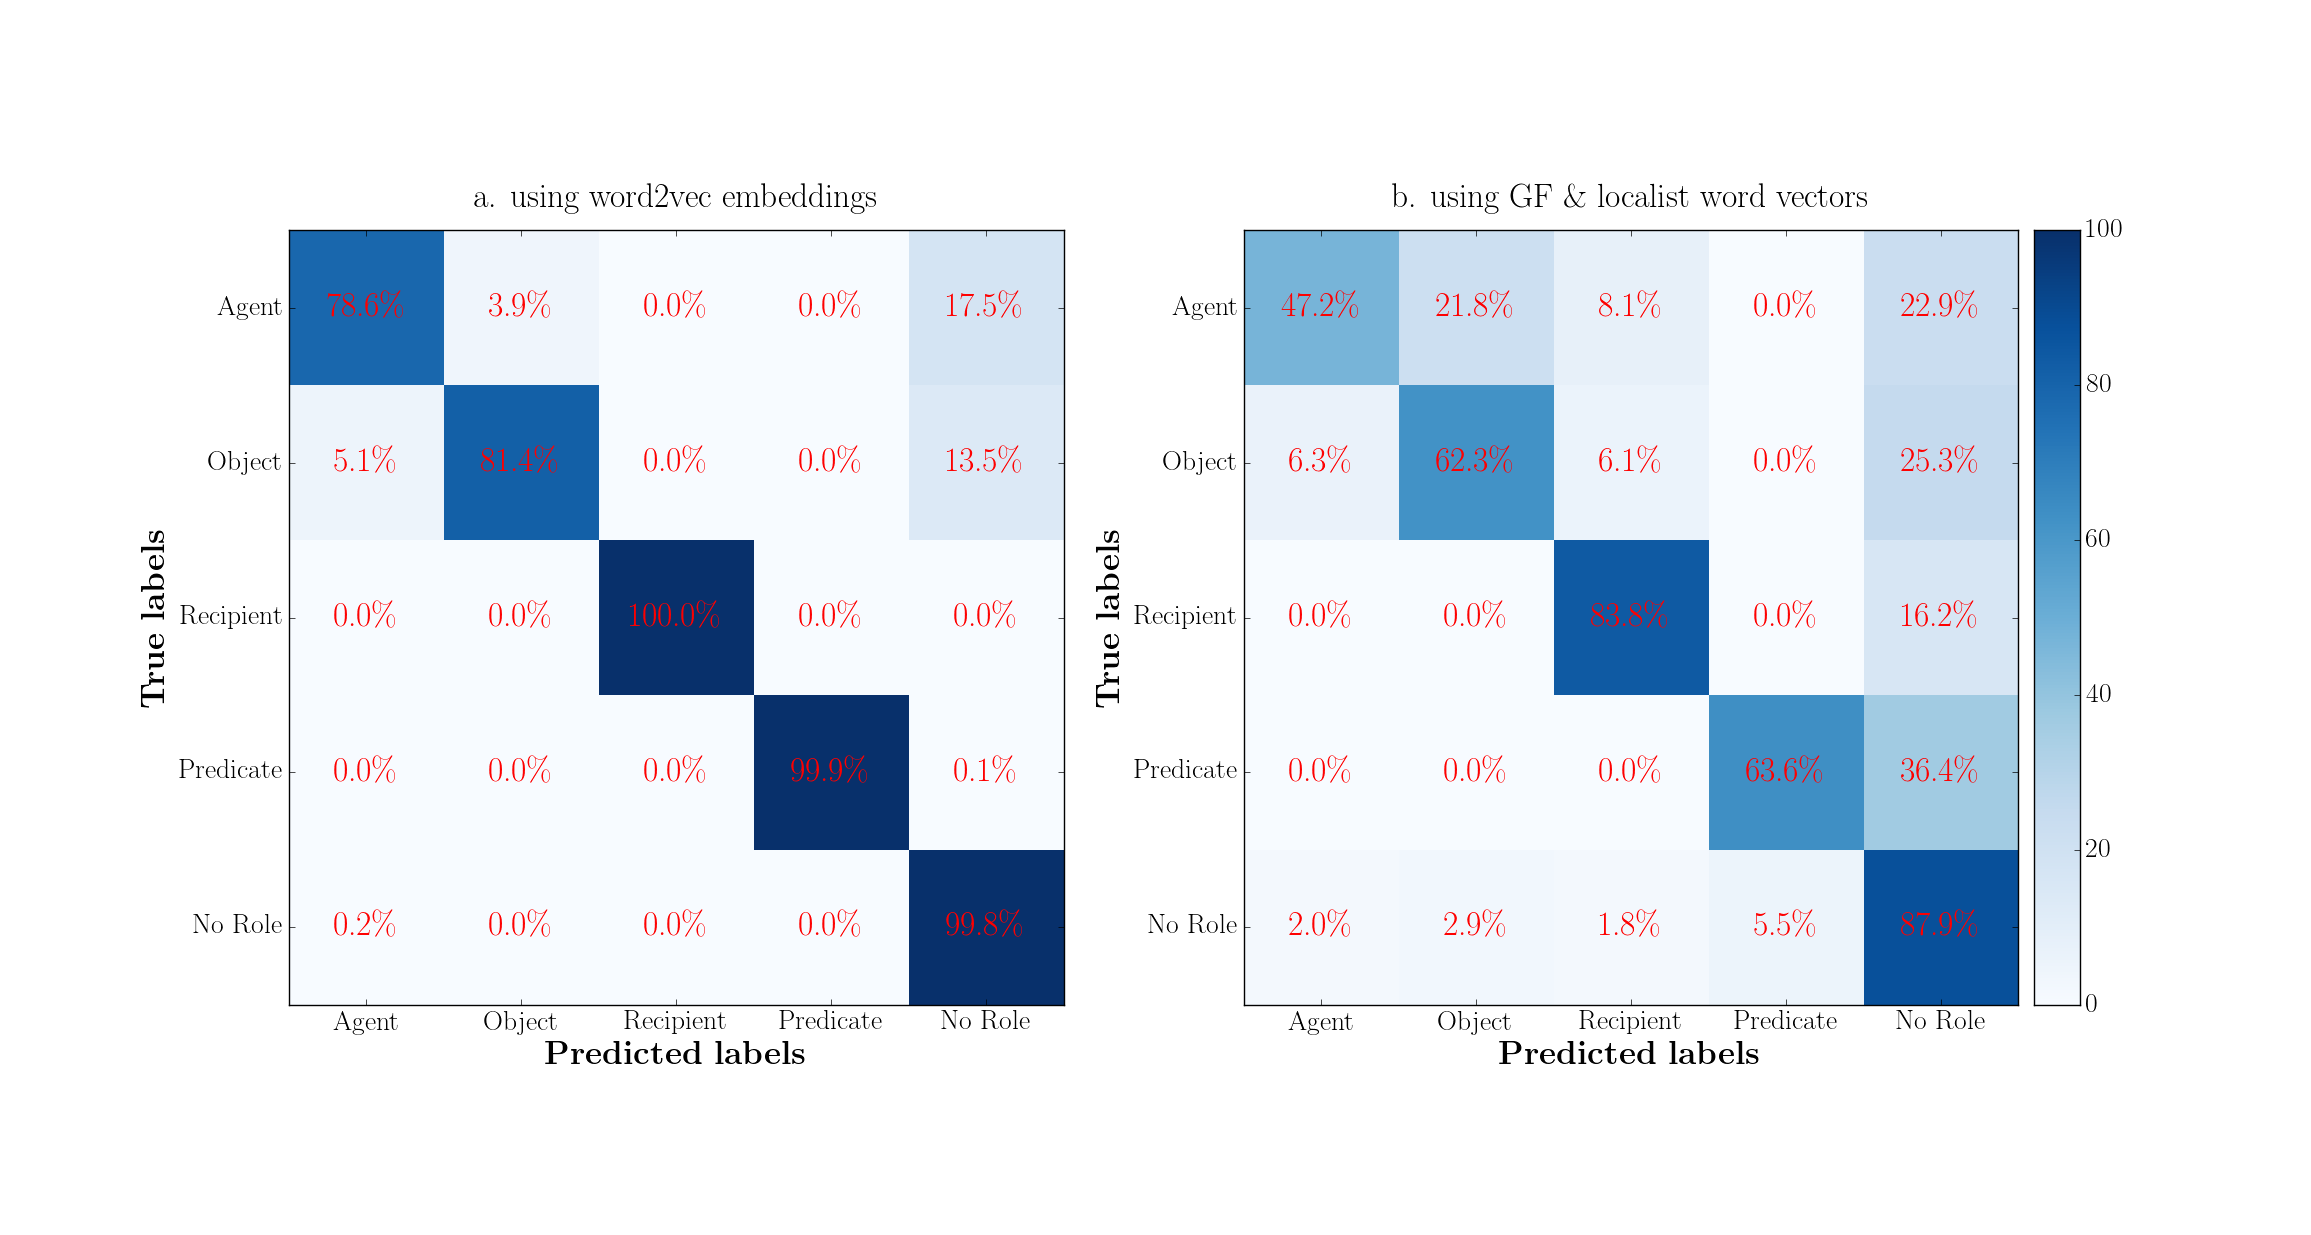
\includegraphics[width=1.0\linewidth]{confusion_matrix}
\caption[Normalized confusion matrix on corpus 462 with Word2Vec-ESN model variant] {\textbf{Normalized confusion matrix with Word2Vec-ESN model variant:} The confusion matrix with true roles (in rows) and predicted roles (in columns). The top-left to bottom-right diagonal shows the percentage of words whose roles are predicted correctly. Everything other than this diagonal represents the incorrect prediction of roles. Model identified almost all words labelled as Recipient , Predicate and No Role and made some errors in predicting role Agent and Object. The results were obtained with reservoir of 1000 neurons and 10 fold-cross validation.}
\label{fig:confusion_matrix}
\end{figure}


\subsection{Experiment-3: Effect of Corpus structure} 

Recall that the sentences in the corpus-462 were created based on context-free grammar. Thus the sentences in the corpus contain an inherent grammatical structure. The model is thus possibly utilizing the underlying grammatical structure to some extent for learning and generalizing. To test this hypothesis and to demonstrate that the model is not generalizing on any other inconsistent regularity in the corpus, we removed the inherent grammatical structure from the sentence in the corpus by randomizing the word orders within the sentences \cite{xavier:2013:RT}. Such a test will also help us to have insight on what the model is actually learning and whether the model is overfitting or not. The situation of overfitting typically occurs when the corpus size is significantly less than the number of trainable parameters \cite{xavier:2013:RT}. The Word2Vec-ESN model with the reservoir of size 1000 neurons and 42 readout neurons have 42000 $(42 \times 1000)$ trainable parameters, whereas the model variant with reservoir size $1000$ and $5$ readout neuron the trainable parameters are 5000 $(5 \times 600)$. In both the case, the number of trainable parameters is significantly greater than our corpus size (i.e. 462 sentences). This is thus a possible situation of overfitting.

We presented the corpus with the scrambled sentences (i.e. in absence of any grammatical structure) to both Word2Vec-ESN model and its variant. Keeping the reservoir parameters same as used in Experiment \ref{exp-2}, a 10 fold cross-validation was performed. The cross-validation errors obtained in the previous experiment on the corpus-462 with inherent grammatical structure can then be compared with the cross-validation error obtained while using scrambled corpus. If the model is not overfitting and learning from the grammatical structure then the model should not perform better on the corpus with scrambled sentences (i.e. in absence of grammatical structure). However, in the case of overfitting the generalization effect on the corpus should not vary much both in presence and absence of grammatical structure.

\paragraph{Word2Vec-ESN model: } As illustrated in table \ref{tab:corpus-462_errors}, we observed that when using the scrambled corpus as an input to the Word2Vec-ESN model, the model learned with low error rates of $ME = 7.32 \%$ and $SE = 30.30 \%$ in SCL mode, but while testing, it generated cross-validation error rates of $ME = 69.76 \% $ and $SE = 99.13 \%$. Whereas similarly in SFL model the model learned with low error rates i.e. $ME = 9.14 \%$ and $SE = 31.16 \%$  but during cross validation resulted into high error rates i.e. $ME = 67.54 \%$ and $SE = 99.34 \%$. Thus in both the learning modes the model failed to genereralize on the scrambled corpus, whereas it generalized well with unscrambled corpus (see experiment \ref{exp-2} and table \ref{tab:corpus-462_errors) indicating that the model learns the coded meaning of sentences by expoloiting the structure of sentence and not any random regularity in the corpus.

\paragraph{

\subsection{Experiment-4: Effect of Reservoir size}

The most important hyperparameter which effects the performance of the model is the size of the reservoir (i.e. number of neurons in the reservoir). Addition of neurons in the reservoir is also computationally inexpensive because the read-out weights ($W^{out}$) scales linearly with the number of neurons in the reservoir \cite{esn:learn_gs}. So, in order to determine the effect of reservoir size on the performance of the Word2Vec-ESN model and its variant, the simulations were performed over a range of reservoir size. For this experiment we used the same optimal reservoir parameter identified in the experiment \ref{exp-2} i.e. $ SR = 2.4$, $IS=2.5$

\paragraph{Word2Vec-ESN model: } Figure \ref{fig:reservoir_size_1}) shows the effect of reservoir size on the cross-validation errors rates (i.e. meaning and sentence error). It was observed that both the meaning and sentence cross-validation error rates reduces with increase in reservoir size but asymptotes when the reservoir size is above 1000 on corpus-462. This indicates that the model can not generalize further for this corpus with further increase in reservoir size. However, the lowest errors were observed in the reservoir with 2882 neurons with meaning and sentence error of $6.74 \% (\pm 1.5\%)$ and $17.39\% (\pm 4.23 \%)$ in SCL mode and $8.70 \% (\pm 1.62\%)$ and $22.60\% (\pm 5.25 \%)$ meaning and sentence error in SFL mode respectively. It can be noticed that the lowest error do not vary significantly when compared to errors obtained with the reservoir of size 1000 neurons (see table \ref{tab:corpus-structure}).

\begin{figure}[hbtp]
\centering
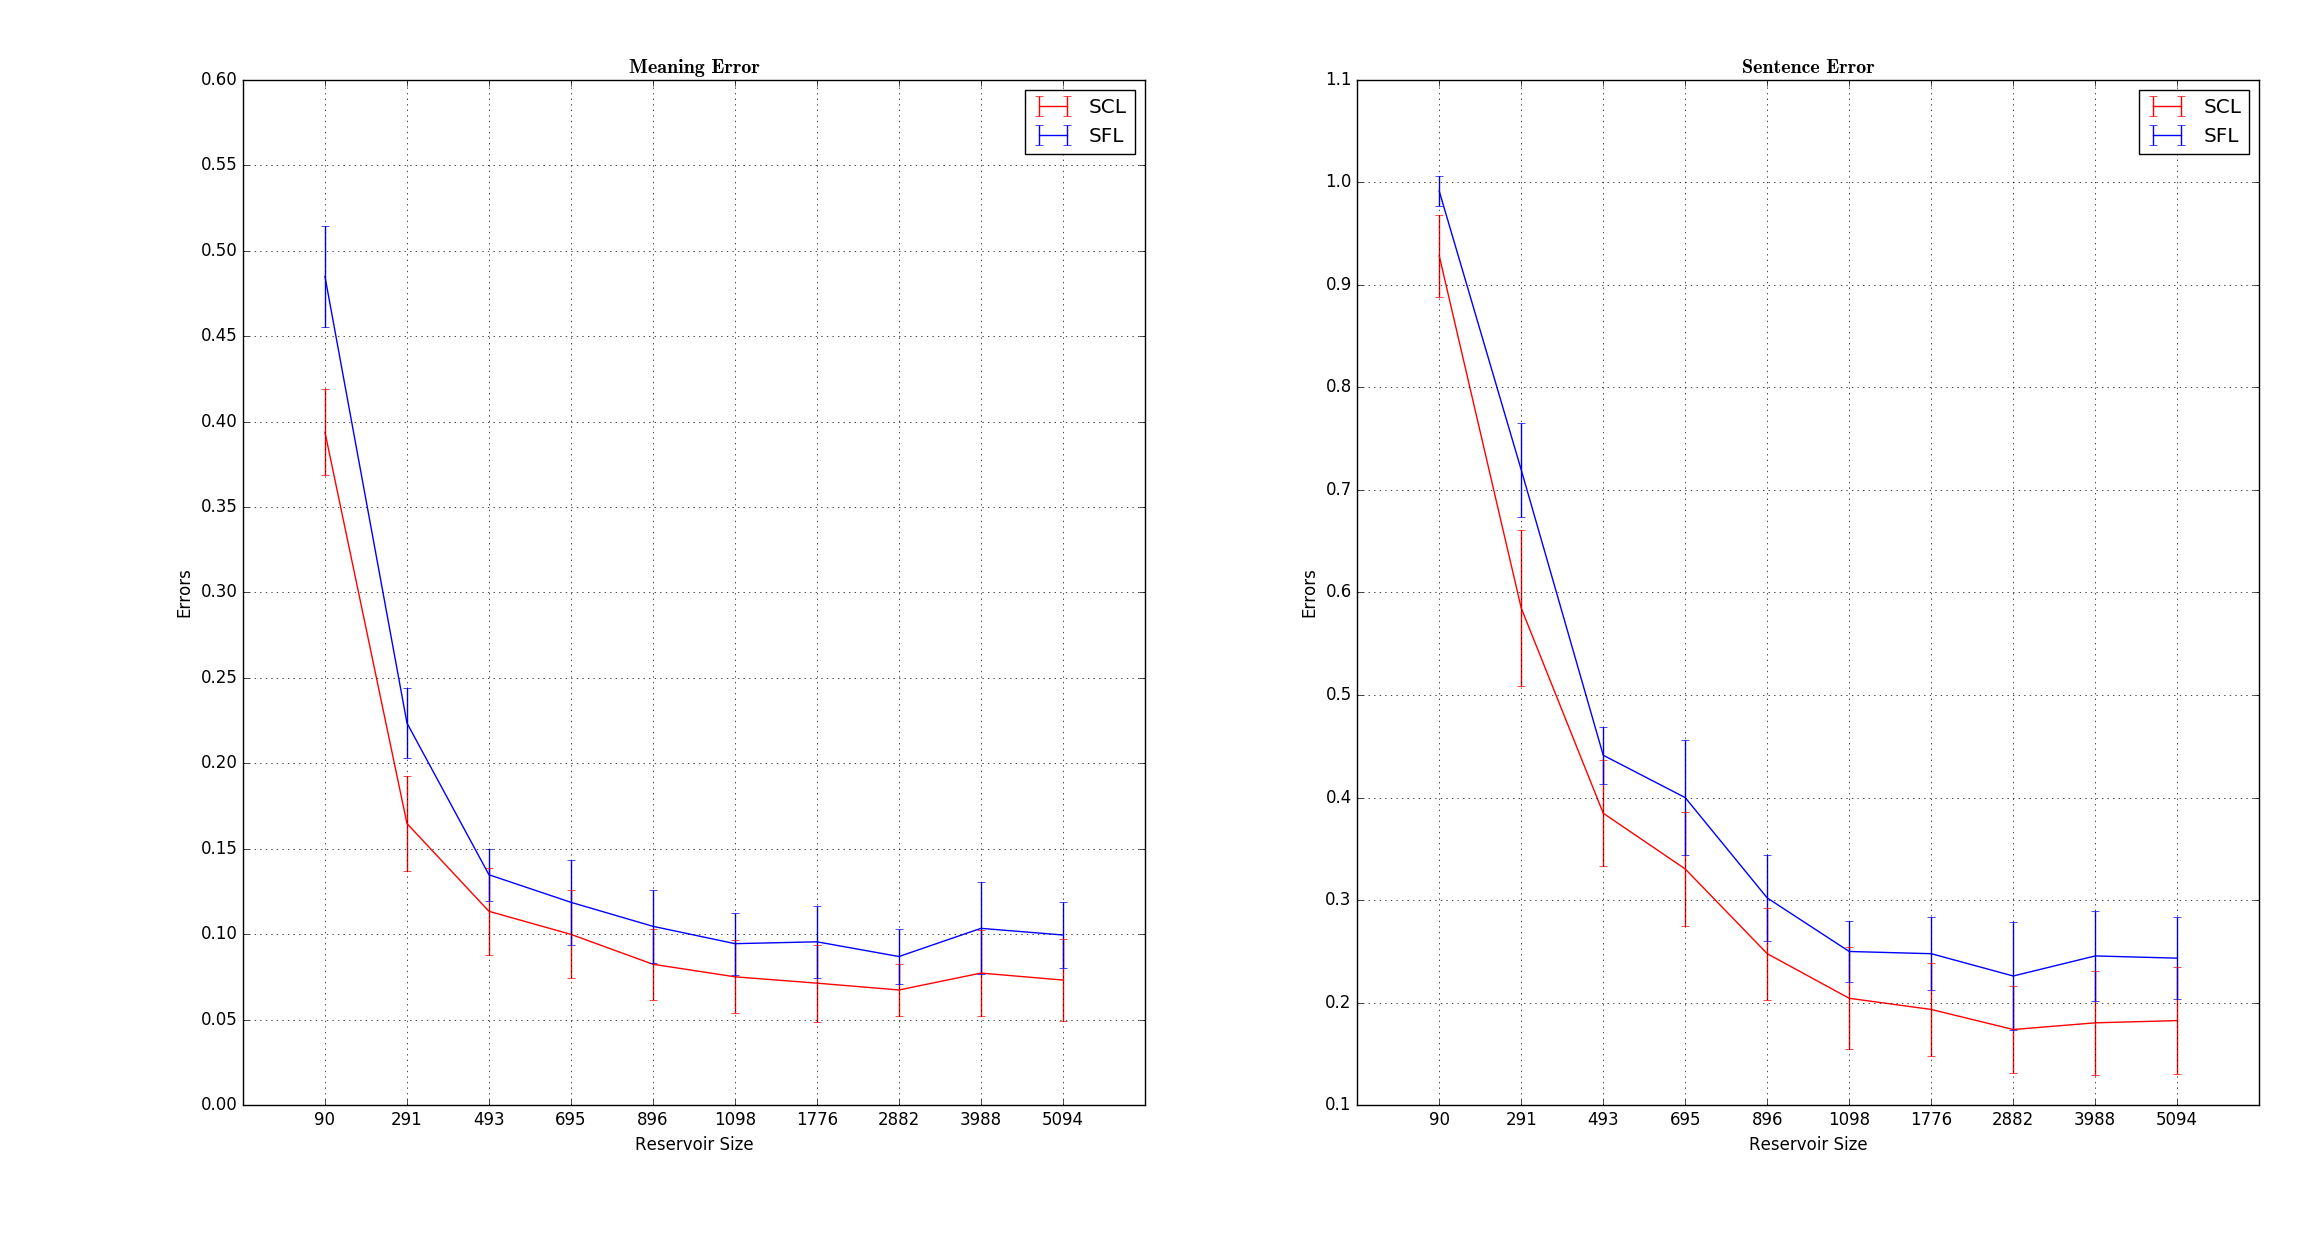
\includegraphics[width=1.0\linewidth]{reservoir_size_1}
\caption[Effect of reservoir size on Word2Vec-ESNM model]{\textbf{Effect of reservoir size on cross validation errors on Model Variant-1:} Description goes here.}
\label{fig:reservoir_size_1}
\end{figure}

We also studied the effect of reservoir size on the performance of model variant, when using word2vec word embeddings and also when using grammatical construction of sentence along with localist word representation. In figure \ref{fig:reservoir_size_2}, it can be clearly observed that the model variant performs much better with word2vec word embeddings with all reservoir size when compared to use grammatical construction of sentence with localist word vector. Even the highest F1-Score ($F1 = 80.06 \%$) obtained using localist representation with reservoir size 2250 is much less than that of obtained using word2vec word embeddings with reservoir of size 200 (F1 = $ 93.56\%$). Overall with increase in reservoir size the classification scores also increases irrespective of the word vectors used as an input to the model. The model also asymptotes when reservoir size is 200 and 600 with word2vec and localist vectors respectively, indicating that model can not be genralized further on the corpus-462). 

\begin{figure}[hbtp]
\centering
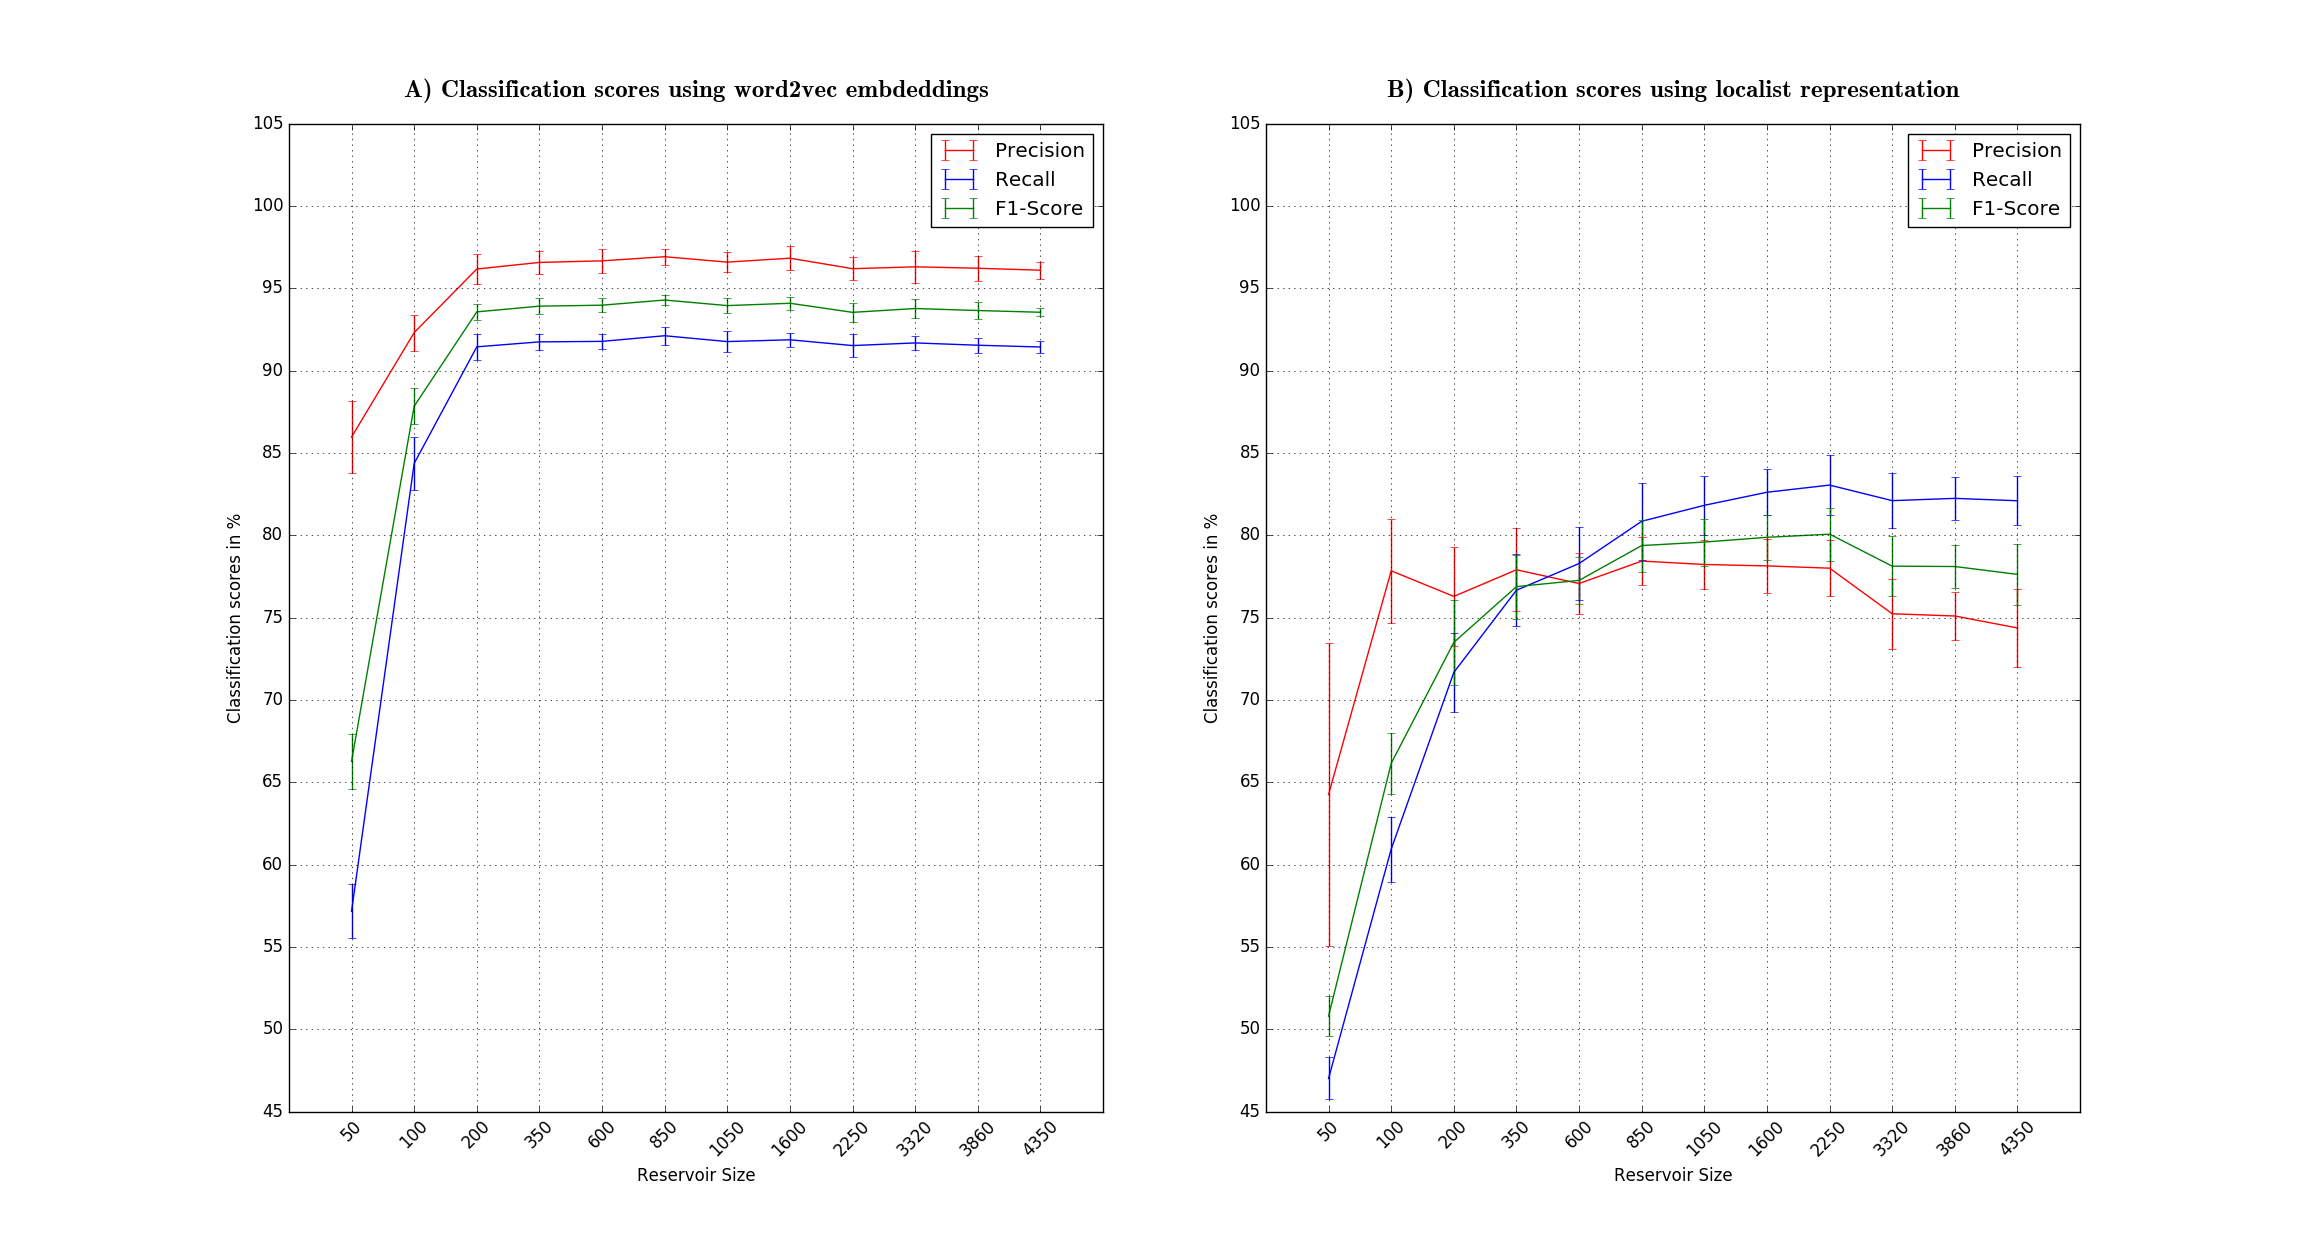
\includegraphics[width=1.0\linewidth]{reservoir_size_2}
\caption[Effect of reservoir size on Word2Vec-ESNM model variant]{\textbf{Effect of reservoir size on classification scores of Model Varinat-2:} Description goes here.}
\label{fig:reservoir_size_2}
\end{figure}

\subsection{Experiment-5: Effect of Corpus size}

In the previous experiments we noticed that the errors rates with Word2Vec-ESN model and classification scores model variant [] improved as we extended the corpus size from 45 to 462 sentences. To investigate the effect of corpus size and scaling capability of the model, we used extended corpus-90582(see section) for this experiment. As the corpus also contains $12\%$ of ambiguous sentences which impede the learning and generalization of the model, this experiment will also validate the model's ability to process the abmbiguous sentences.

In order to study the generalization capabilty of the model with different corpus size,  6 sub-corpora were created by randomly sampling $6\%$, $12\%$, $25\%$, $50\%$, $75\%$, $100\%$ of sentences from the orginal corpora of 90582 sentences\cite{end-to-end}. Each of the sub-corpora was exposed to the model and 2-fold cross validation is performed where the model was trained on half the sub-corpora size and tested on remaining half. The second half used for testing was then used to train the model and then tested on the first half used for training previously.

Figure \ref{fig:corpus_size_1} shows the cross validation errors rates with respect to corpus size while using model variant-1. It can be observed that with increase in corpus size from $6 \%$  to $25 \%$, the meaning error sharply drops from some $12.23 \%$ to $3.92 \%$ in SCL mode and from $12.10\%$ to $4.88 \%$ in SFL mode. Similarly, the sentence error also decreases from $54.43 \%$ to $21.89 \%$ in SCL and from $55.22 \%$ to $26.17 \%$ in SFL mode. When the sub-corpora size is $50\%$, where the model was trained only on $25\%$ of corpora size, the model already generalized with $17.11 \%$ sentence error and $2.98 \%$ meaning error in SCL mode and  $22.32 \%$ sentence error and $4.13 \%$ meaning error in SFL mode. The more gradual slope from $50 \%$ to $100 \%$ sub-corpora size in both the learning modes for meaning and sentence error indicates the model has already generalized and further increase in corpus size won’t have much effect on cross validation error.
 

\begin{figure}[hbtp]
\centering
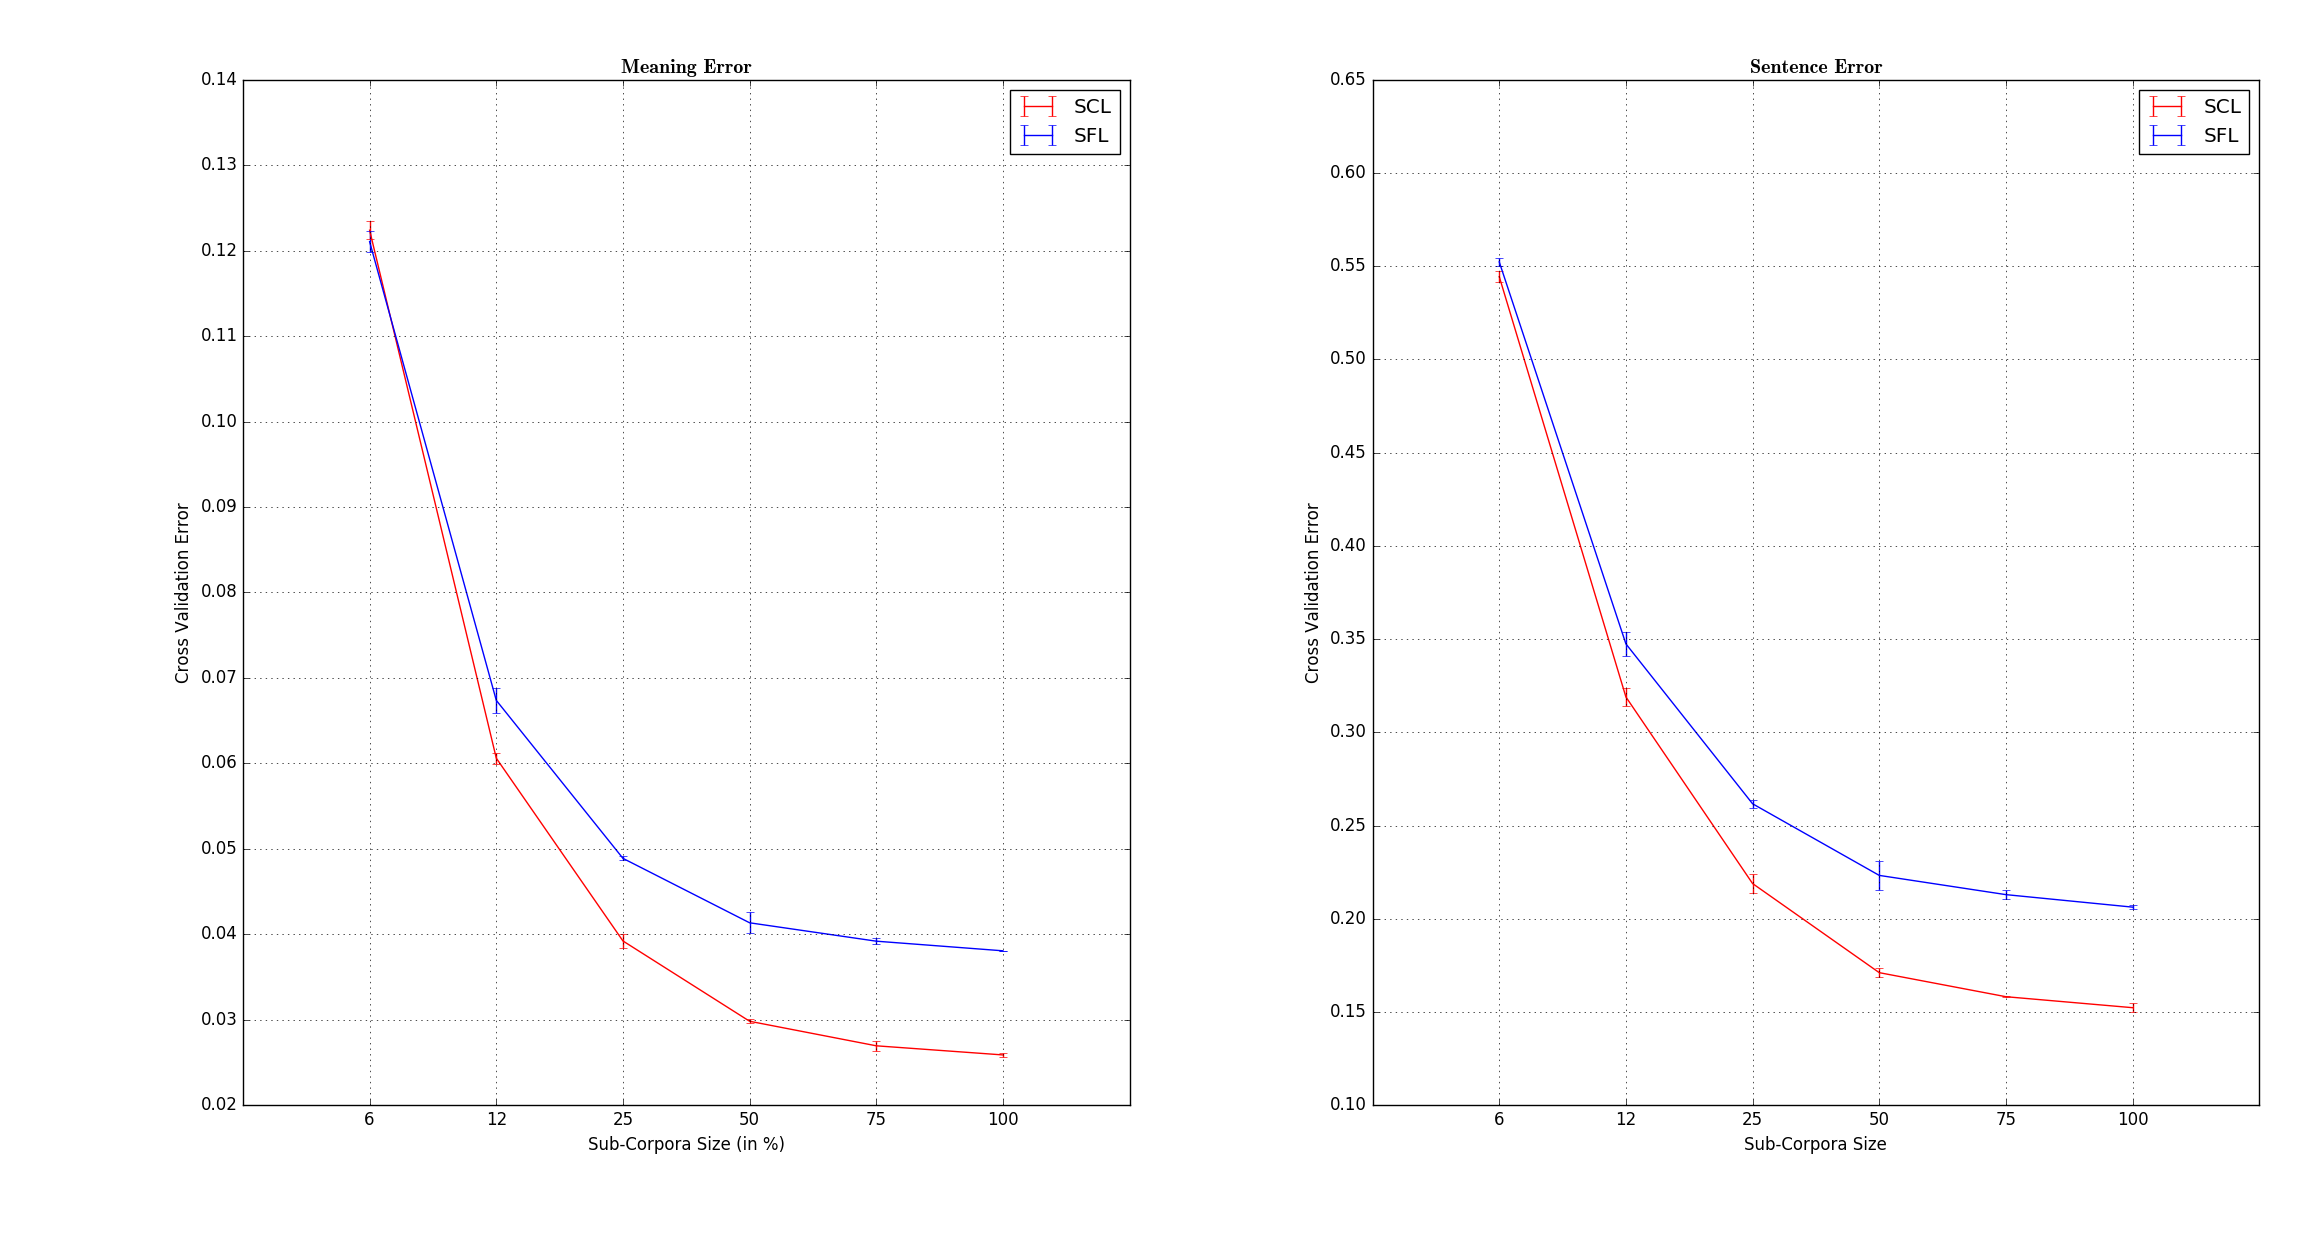
\includegraphics[width=1.0\linewidth]{corpus_size_1}
\caption[Effect of corpus size on Word2Vec-ESN model]{\textbf{Effect of corpus size on cross validation errors:} Description goes here.}
\label{fig:corpus_size_1}
\end{figure}


\begin{figure}[hbtp]
\centering
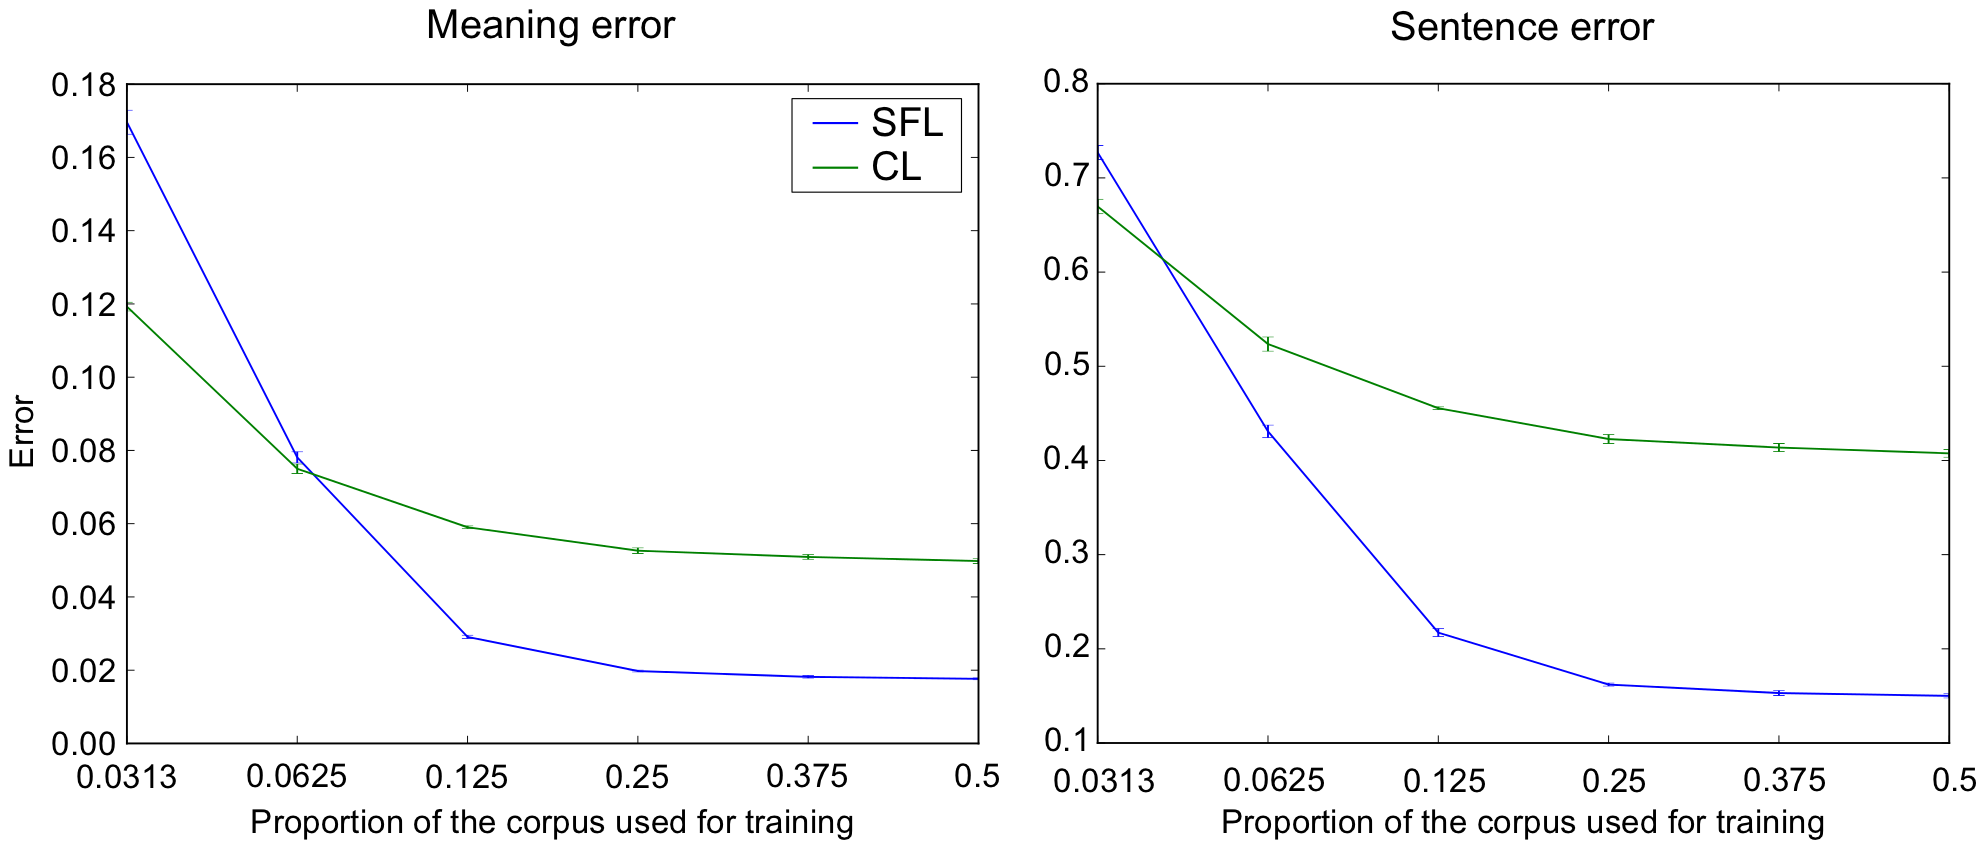
\includegraphics[width=1.0\linewidth]{corpus_size_xavier}
\caption[Effect of reservoir size on Word2Vec-ESNM model variant]{\textbf{Effect of corpus size on cross validation errors using localist word vector as reported in [ref?]:} Description goes here.}
\label{fig:corpus_size_xavier}
\end{figure}


\newpage

\subsection{Experiment-6: Neural output activity of the model}

In the previous experiments we observed that both the model variants generalized well and cross validation error rates dropped with increase in reservoir size. As we saw that model variants performs better when we increased corpus size from 45 sentences to 462 sentences. As corpus-45 contains sentence with uniques grammatical structure (i.e. active, passive, subject and object relative etc.) we added these 45 sentences to corpus-462 so the resultant corpus have 507 sentence (462+45) and analysed the activation produced by model variant-1 for the input sentences. We observed that while learning the model is re-analyzing the thematic roles across the time. The same behaviour was observed by xavier et. al [ref?] with sentences in grammatical constructions form and localist representation of words. However we observed that the model is making earlier predictions with word2vec embeddings. The reason for such a behavior is because the word2vec word embeddings were learned from the context words and each word vector encodes the information about neighbouring words. 

We examined and plotted the four sentences with active and passive constructions studied in Hinaut et al. [ref].

\begin{enumerate}[noitemsep]
\item the man gave the book to the boy. \label{eg-1:or-sent-17}
\item the man took the ball that hit the glass. \label{eg-1:or-sent-23}
\item the boy caught the ball that was thrown by the man.  \label{eg-1:or-sent-27} 
\item the ball was pushed by the man.  \label{eg-1:or-sent-16}
\end{enumerate}

Figure \ref{fig:act_analysis_1} shows the activations for these four different sentences across time. As all the four sentences start with "the", activation at this word is same for all the sentences. In sentences \ref{eg-1:or-sent-17} and \ref{eg-1:or-sent-23} with the arrival of first noun (i.e. man) the activation of noun-2 (i.e. book and ball) being an object of verb-1 is increased and confirmed with arrival of verb 'gave' and 'took' respectively.

\begin{figure}[hbtp]
\centering
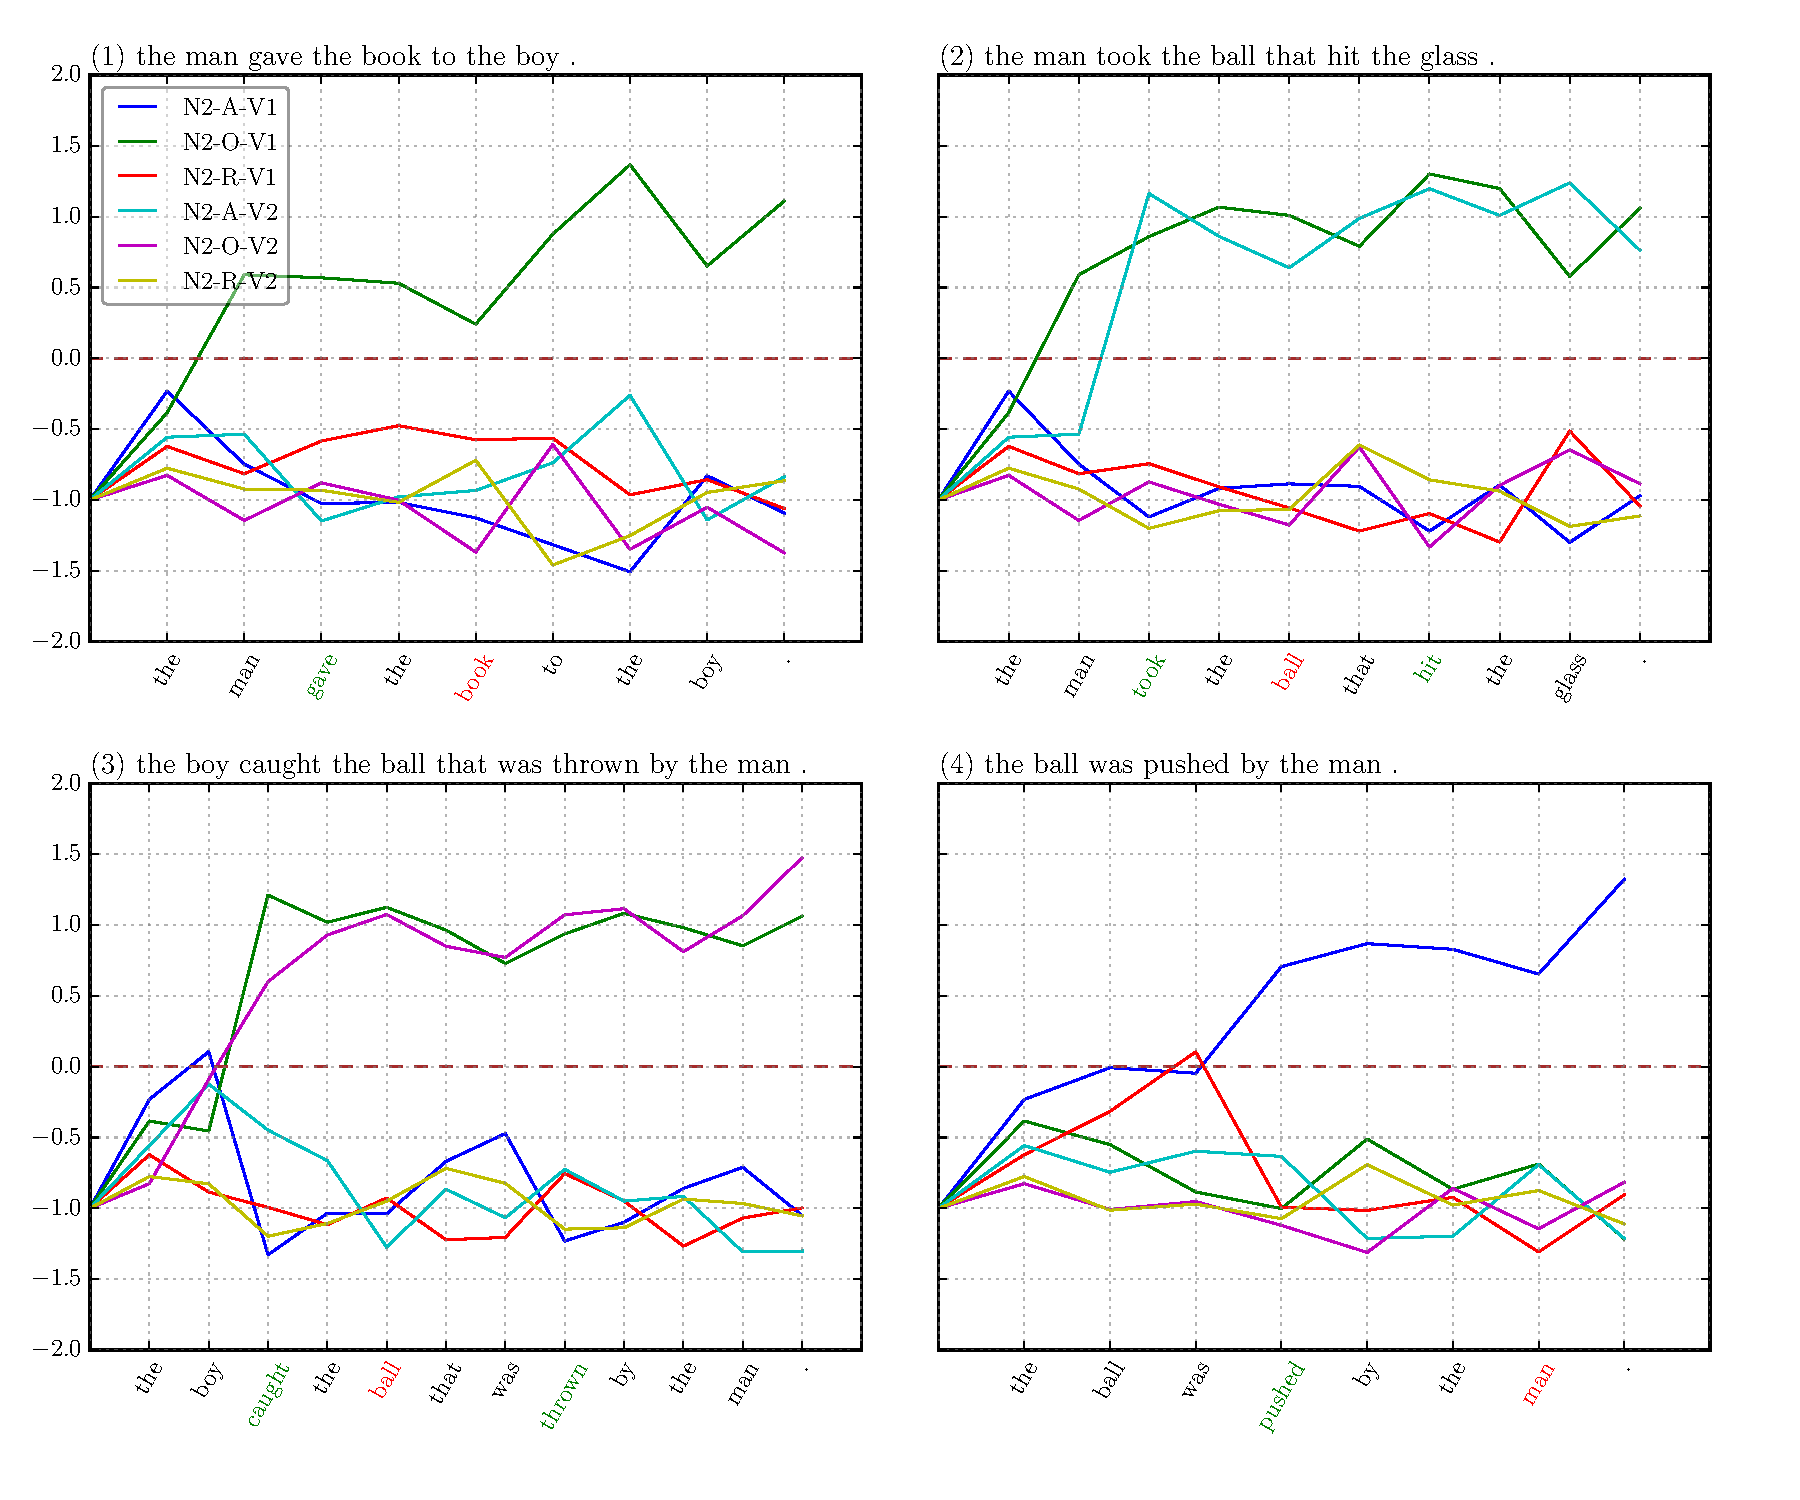
\includegraphics[width=1.0\linewidth]{act_analysis_1}
\caption[Online Reanalysis of activation by Language model:]{\textbf{Online Reanalysis of activation by Language model:} Description goes here.}
\label{fig:act_analysis_1}
\end{figure}

Consider another two sentences 
\begin{enumerate}[noitemsep]
\item the dog that chased the cat ate the rat \label{eg-1:or-sent-17}
\item the cat that the dog chased bit the man. \label{eg-1:or-sent-23}
\end{enumerate}


\begin{figure}[hbtp]
\centering
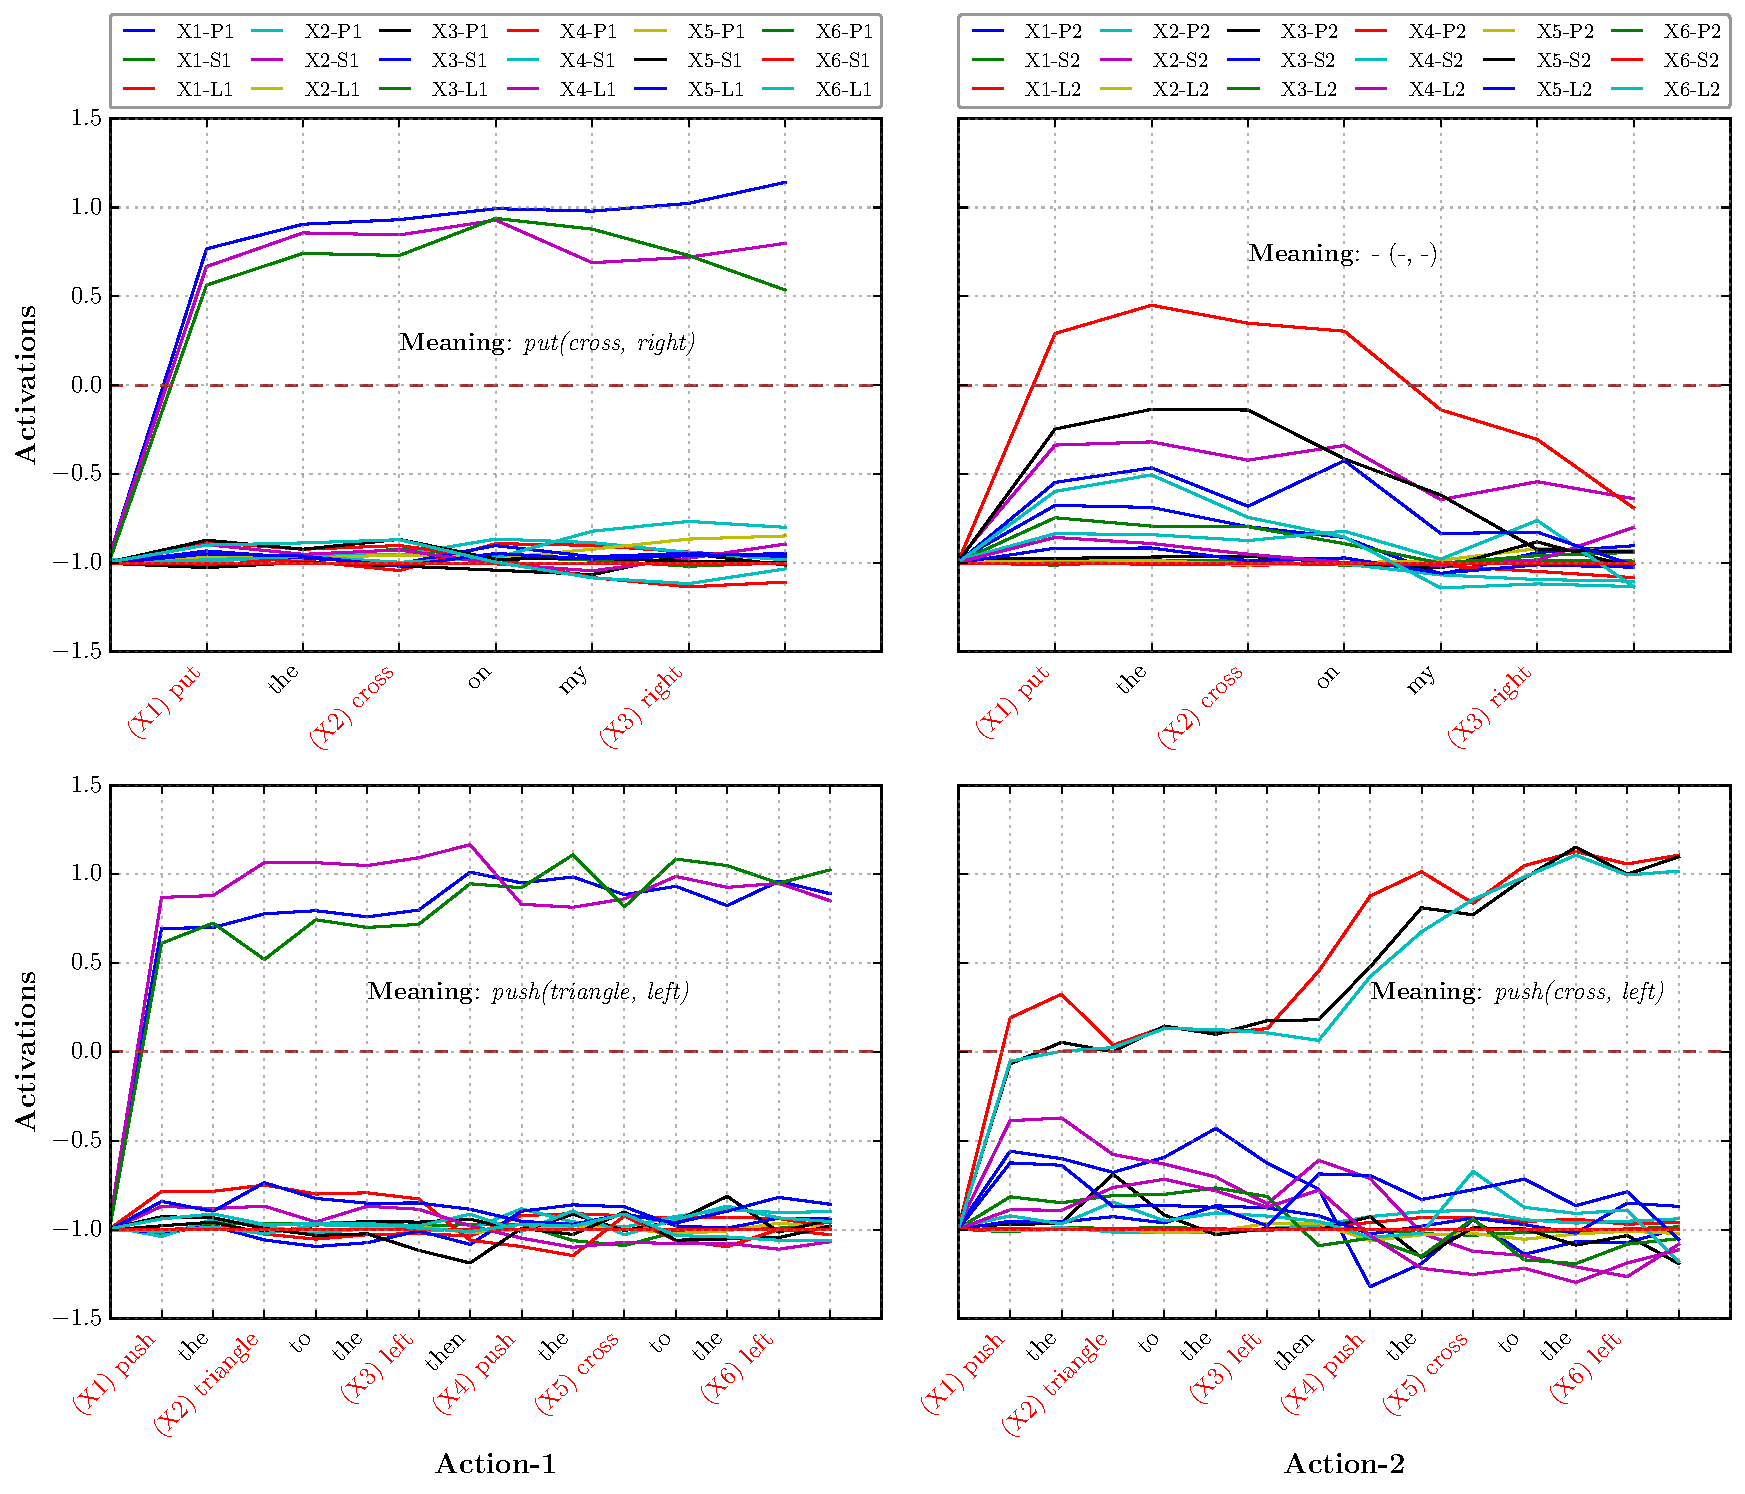
\includegraphics[width=1.0\linewidth]{act_analysis_2}
\caption{\textbf{Effect of corpus size on cross validation errors using localist word vector as reported in [ref?]:} Description goes here.}
\label{fig:act_analysis_2}
\end{figure}

\begin{figure}[hbtp]
\centering
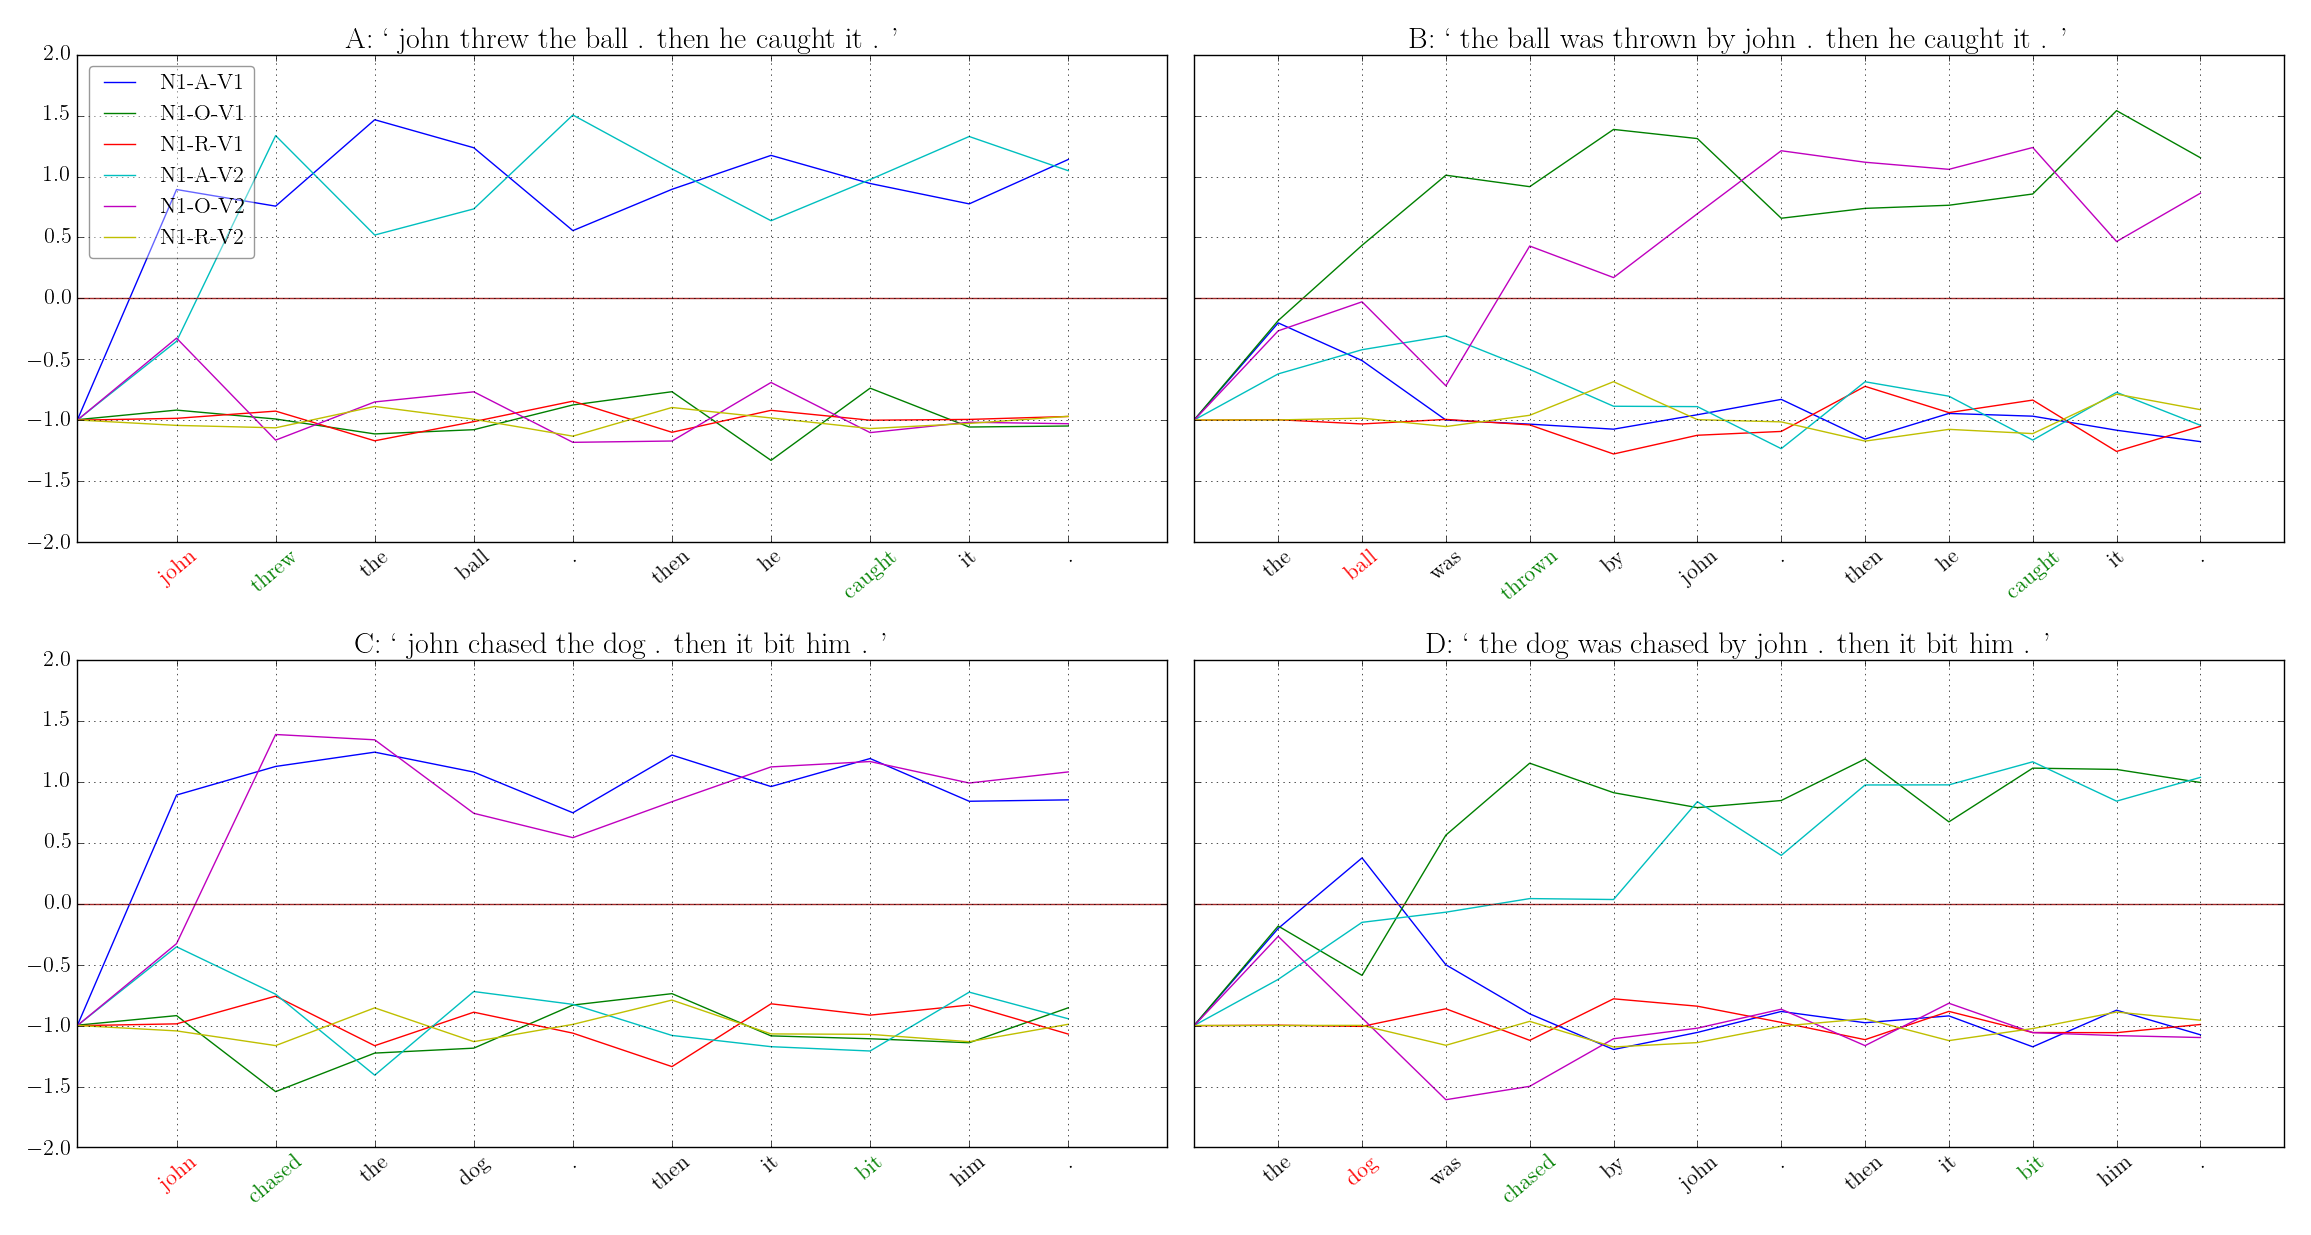
\includegraphics[width=1.0\linewidth]{act_analysis_3}
\caption{\textbf{Effect of corpus size on cross validation errors using localist word vector as reported in [ref?]:} Description goes here.}
\label{fig:act_analysis_3}
\end{figure}


\subsection{Experiment-7: Generalization on new corpus}

One may argue that the previously used corpus (corpus-462 and corpus-90k), which were artifically constructed using grammer is adding a bias to the model which makes it easier for the model to learn and genralize on these corpus for thematic role assignment task. To answer this question, in this experiment we used the corpus-373 collected by Hinaut et al. \cite{tra:tra:xavier_hri} in a Human Robot Interaction (HRI) study of language acquisition. 

To test the generalization of Word2Vec-ESN model on this corpus, leave-one-out (LoO) cross validation was performed. We chose LoO, so that results can be compared with that of obtained using $\theta RARes$ model of	Xavier et al. \cite{tra:tra:xavier_hri}. As illustrated in table \ref{tab:corpus_373}, it can be observed that while using word2vec word embeddings over grammatical form and localist word vectors, of the input sentence, error improved by $26.31 \%$, $17.97 \%$ sentence error with 500 and 1000 reservoir neurons respectively. It can also be observed that with increase in reservoir size the sentence error also decreases. For this experiment we did not explore for the best parameters, but instead we used the optimized parameter obtained on corpus-462 in experiment 2 i.e. SR = 2.4, IS = 2.5 and LR = 0.07. This shows that previously learned model parameters are capably roboust enough to generalize on the new corpus. 

\begin{table}
\centering
\begin{threeparttable}
\caption[Word2Vec-ESN model generalizing on new coprus]{Generalization error in SCL mode on corpus-373.}
\label{tab:corpus_373}
\rowcolors{2}{gray!25}{white}
\begin{tabular}{llll}
\toprule
Reservoir 	 		& Sentence Error 	&  Word2Vec-ESN 		& $\theta RARes$ \\
\midrule                 
\textbf{500 N}		& mean(std.) 		& 42.65 ($\pm$ 1.36) 	& 68.96 ($\pm$ 2.03)  \\
					& Best 				& 26.54 				& 44.50  \\
\textbf{1000 N}		& mean(std.) 		& 40.29 ($\pm$ 1.13) 	& 58.26 ($\pm$ 1.37)\\
					& Best 				& 25.73 				& 34.85 \\
\bottomrule
\end{tabular}
\begin{tablenotes}
\small
\item 
Sentence errors (in $\%$) obtained with Word2Vec-ESN model and $\theta RARes$ in SCL mode for input sentences with reservoir of size 500 and 1000 neurons. The results reported are mean and standard deviation of 10 reservoir instances. The best error here means the count of sentence errors common in all 10 reservoir instances\cite{tra:xavier_hri}.  
\end{tablenotes}
\end{threeparttable}
\end{table}